\chapter{基于曼哈顿切线距离的指纹定位算法}
\label{cha:fingerprint}

本章将介绍基于曼哈顿切线距离的指纹定位算法,用户作为无线蜂窝网或者Wi-Fi信号的接收端,根据接收信号强度实现对自身的定位。虽然信号是在用户终端收集的,但是不必限制定位的解算也必须在本地完成,也可以将收集的信号上传云端,服务器端解算完成后返回给终端。本章所提出的算法就是一种需要在云端完成计算的算法。

\section{指纹定位中的常用距离度量方式}

指纹定位是基于一种假设,即在物理空间中邻近的两点,在信号空间中的距离也应较短,反之亦然,因为物理上相邻的两点应有相似的信道信息和多径效应。所以,如果从多个不同WAP发射信号的RSS已知,物理位置应该可以通过在信号空间中与历史数据运算估算出当前位置。K近邻(K-Nearest Neighbors, KNN)算法是一种常见的用于指纹定位的机器学习算法,通过在信号空间中找出最近的k的点并以某种方式对这k个点的物理位置组合后得到估测的定位。本文所采用的的算法是加权KNN(Weighted-KNN),即以信号空间中距离的倒数作为权重对物理位置加权平均得到定位。KNN算法中最明显的可调节参数就是近邻数k,但是既然近邻是由距离度量的,因此距离度量方式也应当被认真选择。

\subsection{常见度量方式}

首先,让我们定义一个物理-信号空间对:$(\mathbf{x}, \mathbf{s})$,其中$\mathbf{x}$是物理空间坐标,$\mathbf{s})$是不同WAP到终端的RSS向量。不妨假设$D$代表信号向量$\mathbf{s}$的维度。

正如第\ref{cha:intro}章中所说,欧氏距离、曼哈顿距离和余弦相似度是指纹定位中一些常用的度量方式。

欧氏距离和曼哈顿距离都属于明可夫斯基距离(Minkowski Distance),由下式定义:
\begin{equation}
d_{minkowski}(\mathbf{s}, \mathbf{r}) = \left(\sum_{i=1}^{D} {{\left| s_i - r_i \right|}^p}\right)^{\frac{1}{p}}, \label{eq:minkowski}
\end{equation}
其中$\mathbf{s}, \mathbf{r}$是两点的RSS向量。欧氏距离中$p=2$,曼哈顿距离中$p=1$。

经典余弦相似度由下式定义:
\begin{equation}
Cosine(\mathbf{s}, \mathbf{r}) = \frac{\mathbf{s}^T\mathbf{r}}{\left\|\mathbf{s}\right\|\left\|\mathbf{r}\right\|}, \label{eq:cosine}
\end{equation}
其取值于$[-1, 1]$区间,并且该值越接近1,则两个向量越相似,但是这与距离相反,因此我们将以$1 - Cosine(\mathbf{s}, \mathbf{r})$作为度量。

上述3种度量方式将被纳入考量范围,以比较它们的定位误差RMSE。第\ref{sec:exp}节的结果显示,在这些度量方式中,曼哈顿距离能取得最小的RMSE。

\subsection{常用度量方式的弊端}

虽然上述距离度量方式在指纹定位中被广泛应用,但是它们仍然有一些弊端会降低定位精度:
\begin{itemize}
	\item 不同RSS的信号共享相同的权重,这不是一个合理的选择。根据对数距离路径损失函数,在噪声相同的情况下,当RSS较大时,由噪声带来的从WAP到移动终端距离的扰动会小于RSS较小时。比如,同样是由噪声带来1dBM的RSS下降,在RSS较大时反应到距离上的改变就小于RSS较小时。因此,基于较大RSS较大的权重是一种合理的选择。注意到以dBM为单位的信号是自然信号取对数后的结果,那么我们可以逆向这个过程以给予大RSS更大的权重:
	\begin{equation}
	f(\mathbf{s}) = \mathrm{10}^{\frac{\mathbf{s}}{10\lambda}}, \label{eq:exp}
	\end{equation}
	其中$\lambda$是一个控制RSS权重的参数。$\lambda$越小,更大的相对权重会给予大的RSS。如果$\lambda$过小则会使得小的RSS在距离计算中被忽略,而如果$\lambda \rightarrow \infty$则会使得所有RSS的$f(\mathbf{s})$都一样。最终$f(\mathbf{s})$将作为信号空间中的数据,即基于$f(\mathbf{s})$计算K近邻。
	
	巧合的是,这个做法的效果已经被实验证实了~\cite{torres2015comprehensive}。但是,这篇文章没有分析$\lambda$对定位精度的影响,我们的实验结果将在第\ref{sec:exp}节中被展示;
	
	\item 流形的存在。如第\ref{cha:intro}章所述,流形是一个机器学习中的经典假设。样本的微小变化会形成流形,而在指纹定位中,物理空间中邻近的点的RSS应当居于信号空间中的一个流形上,因为局部的小区域应当拥有相似的信道信息而且变化较小。除此之外,在我们的数据集中,可接收信号的基站数量从80到200个不等,相比于二维物理空间,这是一个高维输入,而一般高维数据都居于低维流形上。当流形存在于高维空间中时,两点之间的距离应当是两点所在流形之间的距离而不是简单的距离度量所能表示的。
	
	在流行存在的情况下,如果一个测试点想被准确的分类或者回归,一个简单但低效甚至不可能实现的做法是采集所有可能情况下的数据,这样流形可以自动形成,从而简单度量也可以计算出流形之间的距离。但是,现实中数据集的大小受限,因此需要一种用有限数据估计流形之间距离的算法。
\end{itemize}

\section{指纹定位中的切线距离}

\begin{figure}[tb]
	\centering
	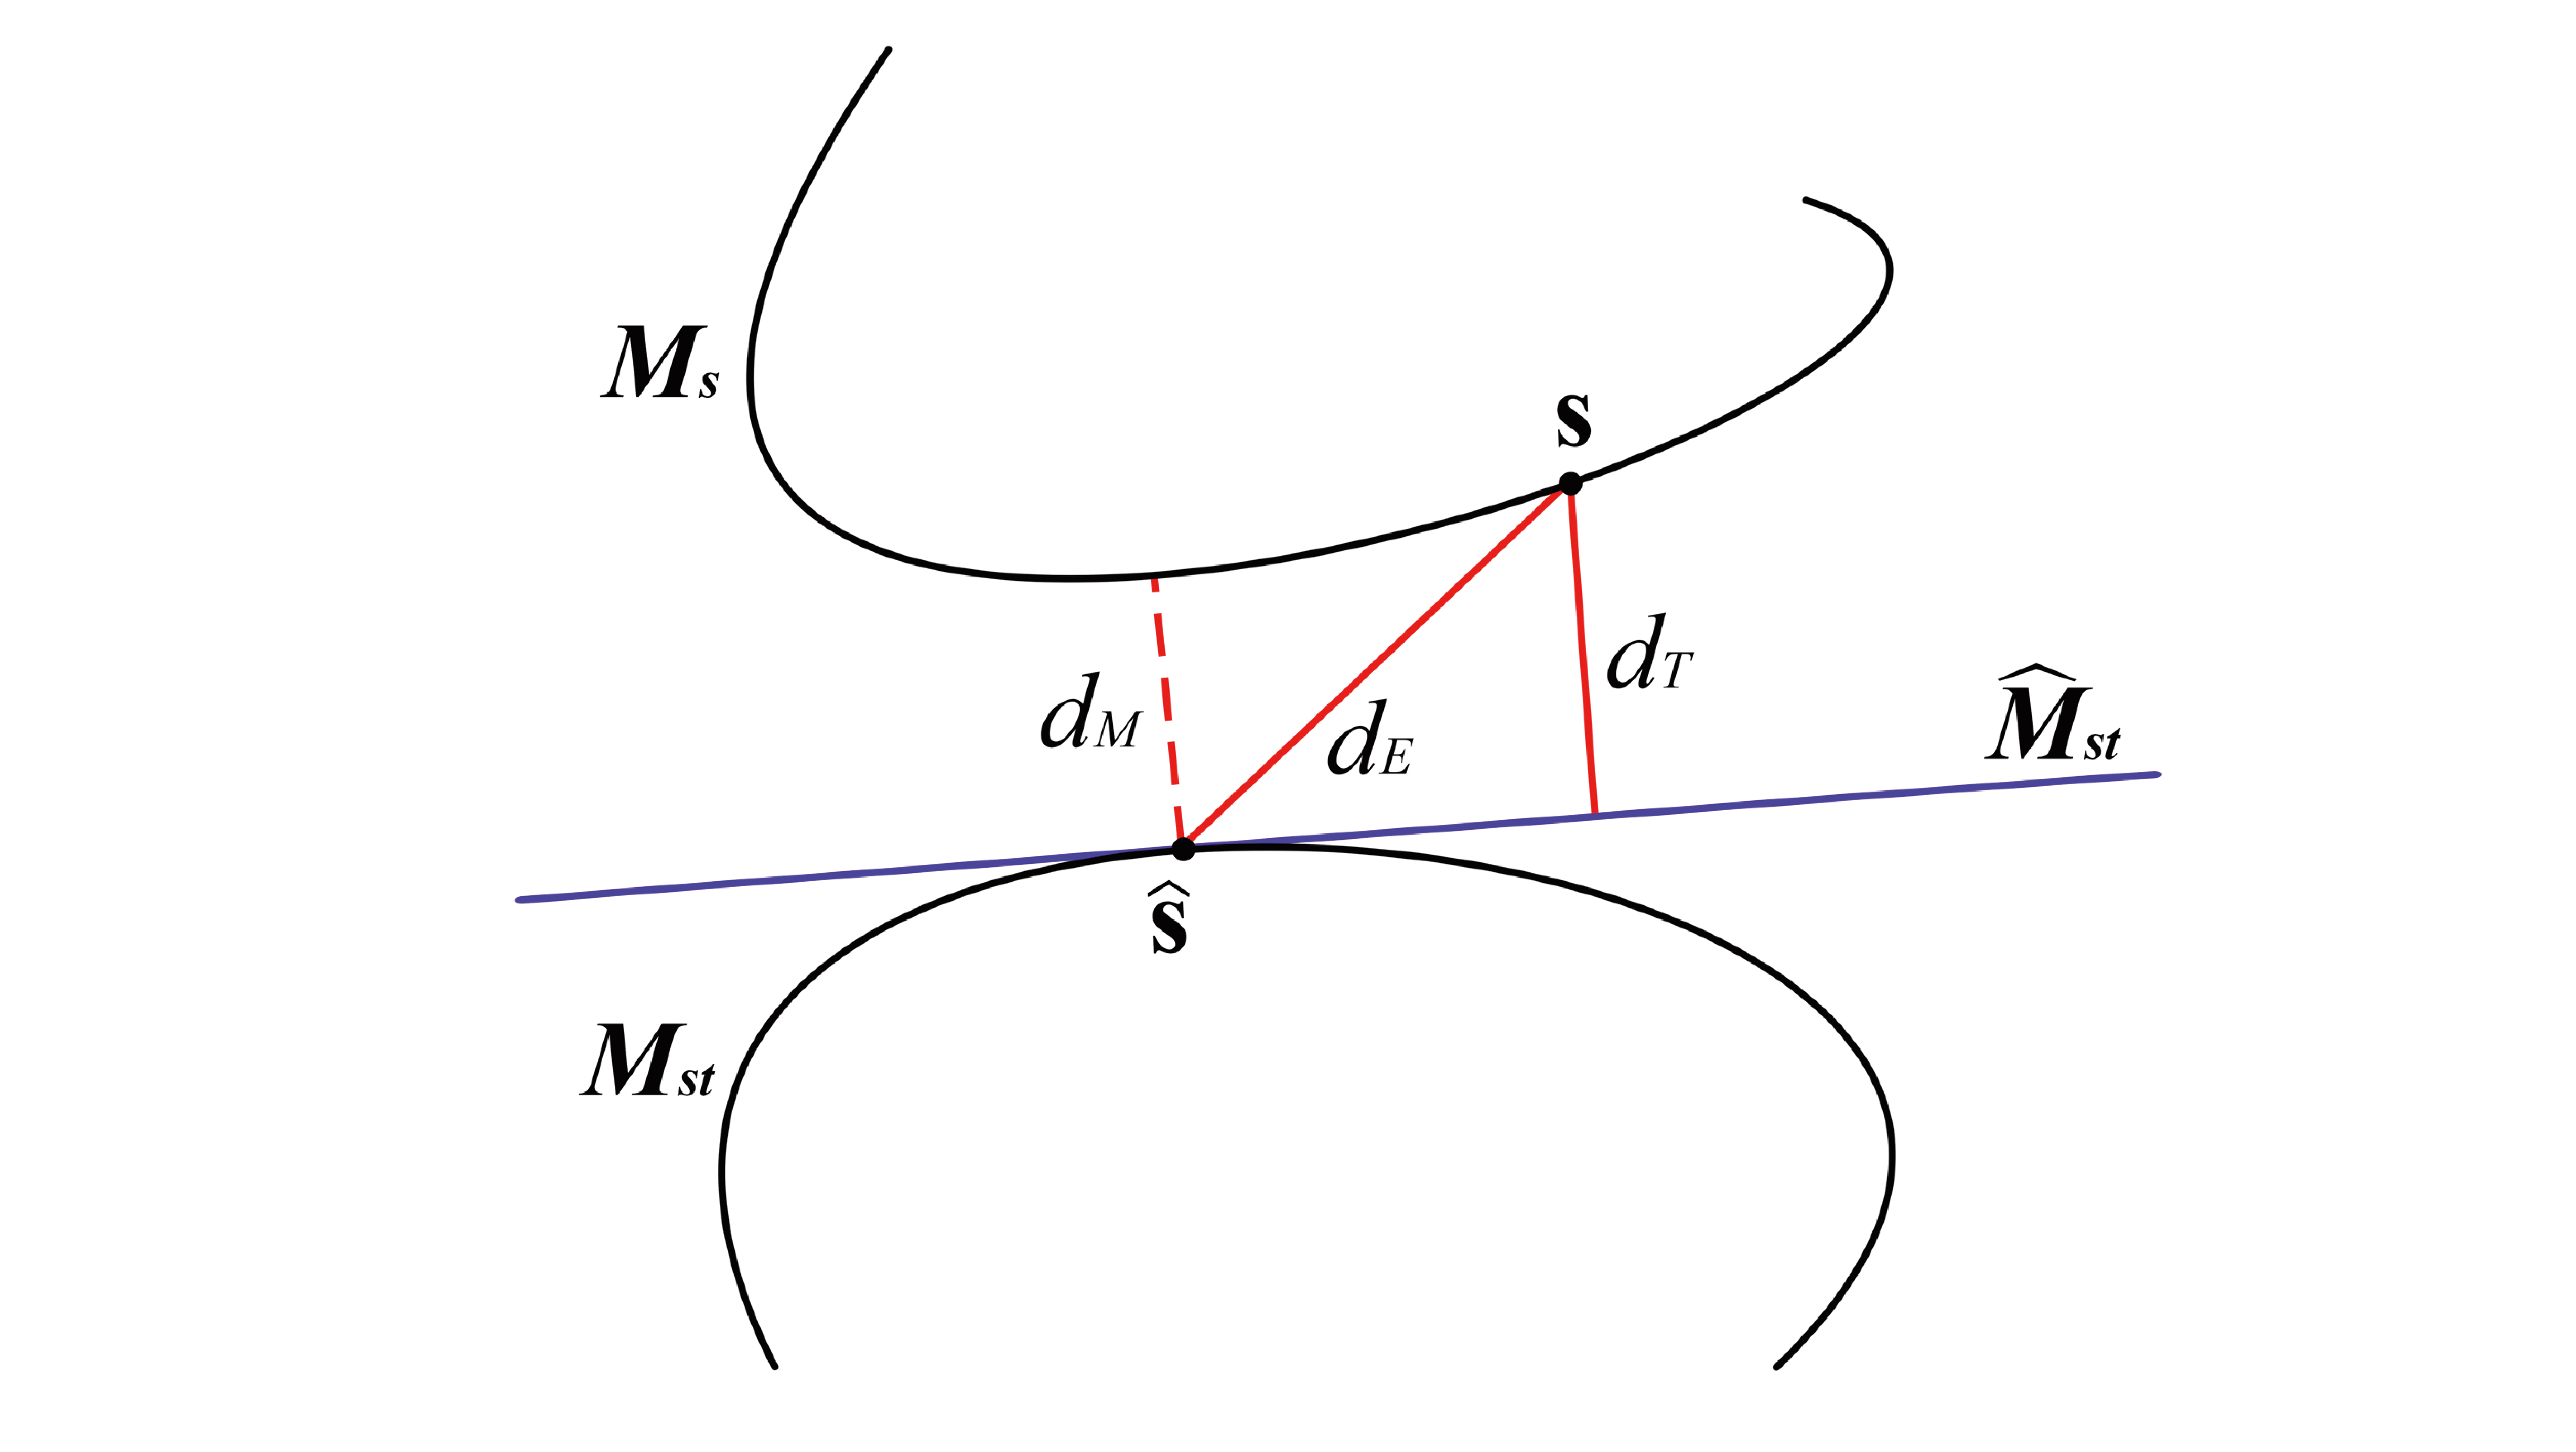
\includegraphics[width=\textwidth]{manifold.pdf}
	\caption{如图展示了欧氏距离、流形间距离和切线距离的关系。在信号空间,$\mathbf{s}$是测试点,$\widehat{\mathbf{s}}$是一个训练点。 $\boldsymbol{M_s}$ 和 $\boldsymbol{M_{st}}$分别是$\mathbf{s}$和$\widehat{\mathbf{s}}$所在的流形。$\boldsymbol{\widehat{M}_{st}}$是$\boldsymbol{M_{st}}$在$\widehat{\mathbf{s}}$处的切线。$d_E$代表$\mathbf{s}$和$\widehat{\mathbf{s}}$之间的欧氏距离。$d_M$代表$\boldsymbol{M_s}$ 和 $\boldsymbol{M_{st}}$两个流形之间的距离。$d_T$代表$\mathbf{s}$到$\boldsymbol{M_{st}}$的切线距离。显然,相比于$d_E$,$d_T$是对$d_M$更好的估计。}
	\label{fig:manifold}
\end{figure}

\textit{切线距离(Tangent Distance)}是一种对测试点到训练点所在流形距离的局部线性近似,从测试点到训练点流形的切线的距离被称作切线距离,如图\ref{fig:manifold}中$d_T$所示。计算切线距离只需要知道$(\widehat{\mathbf{x}}, \widehat{\mathbf{s}})$处的梯度而不是整个流形,因此切线距离的计算所需数据远小于计算流形之间的距离。

理论上,切线的方向与流形的梯度相同。但是由于不知道流形的具体函数从而很难计算梯度,我们将用有限差分获得切线方向。注意到,在我们的场景中,信号空间内的流形由物理空间的微小变化形成,也就是距离的微小变化。比如,如果$(\mathbf{x}, \mathbf{s})$是一个物理-信号空间对,在物理空间中点$\mathbf{x} + a{\bm{\delta}}$在信号空间内的流形 $\boldsymbol{M_s}$上所对应的点应当表示为 $\boldsymbol{M_s}(a)$。$\delta$是一个表征微小变化方向的单位向量,$a$是一个代表由于物理空间变化导致的距离上变化的标量。这种对距离求导数而不是对物理空间坐标求导数的做法看起来并不直接,因为后者的做法更直观且符合常理。原因是物理坐标$\mathbf{x}$是一个二维或者三维向量,意味着求导需要求偏导数。首先,计算偏导数需要更多的计算及时间。更严重的是,用有限差分法估计偏导数需要$\mathbf{x}$中依次只有一个元素微小变化,其他维度的元素不变,而这对于数据采集是一个严峻挑战,尤其是对于大规模室外数据采集。实际上,如果数据采集条件允许,偏导数或者导数对于后续的分析来说没有区别,除了优化变量从标量变成向量了。总之,偏导数依然适用于切线距离。

\subsection{欧式切线距离}

切线距离最初被提出时就是基于欧氏距离~\cite{simard1998transformation},由下式定义:
\begin{equation}
d_T = \mathop {\min }\limits_{a} {{\left\| \mathbf{s} - \mathbf{t}a - \widehat{\mathbf{s}} \right\|}_2}, \label{eq:euctd}
\end{equation}
其中$\mathbf{s}$和$\widehat{\mathbf{s}}$分别是信号空间中的测试点和训练点。$\mathbf{t}$是训练点附近的导数:
\begin{equation}
\mathbf{t} = {\left( \frac{\partial s_1}{\partial d}, ..., \frac{\partial s_D}{\partial d} \right)}^T, i = 1, 2, ..., D,
\end{equation}
其中$d$代表距离。因为导数是由有限差分近似估计的,在训练集中选择另一个点与训练点进行差分运算就变得至关重要。我们的方法是在物理空间中找到距离训练点最近的$N$个近邻,之后$N$个导数可如下计算:
\begin{equation}
\mathbf{t}_j = \frac{\mathbf{s} - \mathbf{s}_j}{d_j}, j = 1, 2, ..., N.
\end{equation}
注意到$\mathbf{t}_j$代表第$j$个导数而不是向量$\mathbf{t}$的第$j$个元素。$d_j$的距离度量方式无关紧要,因为它只会影响导数的尺度而不是方向,而尺度的影响在\eqref{eq:euctd}中优化$a$时会被消除。关于$N$对于定位精度影响的数值实验将在第\ref{sec:exp}节中被分析。

$d_T$可以通过求解一个线性最小二乘法而简单的获得:
\begin{equation}
a_j = {\left( {\mathbf{t}_j}^T\mathbf{t}_j \right)}^{-1}{\mathbf{t}_j}^T\left( {\mathbf{s}} - \widehat{\mathbf{s}} \right), j = 1, 2, ..., N. \label{eq:euca}
\end{equation}
在所有$a_j$都被计算之后,对于根据\eqref{eq:euctd}得到的所有切线距离$d_{Tj}$求均值,而这将被当做指纹定位中KNN的距离度量方式。

我们将上述距离称为\textit{欧式切线距离(Euclidean Tangent Distance, ETD)}。虽然ETD很容易求解,但是数值实验显示曼哈顿距离的定位精度优于前文所提到的所有常见距离度量方式,甚至比ETD效果还好。因为ETD的定位精度高于欧氏距离,也许我们可以推演说基于曼哈顿距离的切线距离会比曼哈顿距离表现更好。因此,下一节我们将提出曼哈顿切线距离。

\subsection{曼哈顿切线距离}

为了表述简洁,在后续部分中,导数$\mathbf{t}$和曼哈顿切线距离$d_{MT}$将不会在右下标标注$j$。类似于\eqref{eq:euctd},曼哈顿切线距离可由下式定义:
\begin{equation}
d_{MT} = \mathop {\min }\limits_{a} {\left\| \mathbf{s} - \mathbf{t}a - \widehat{\mathbf{s}} \right\|}_1. \label{eq:mantd}
\end{equation}
但是对$a$优化并不像\eqref{eq:euctd}那么简单,因为L1-范数的导数是符号函数。不妨定义$\mathcal{L} = {\left\| \mathbf{s} - \mathbf{t}a - \widehat{\mathbf{s}} \right\|}_1$,则
\begin{equation}
\frac{\partial \mathcal{L}}{\partial a} = -\mathbf{t}^T \mathrm{sgn}\left( \mathbf{s} - \mathbf{t}a - \widehat{\mathbf{s}} \right). \label{eq:sgn}
\end{equation}
求解\eqref{eq:sgn}是困难的而且甚至无解。在这种情况下,我们需要一种近似函数来尽可能拟合$\mathrm{sgn}(x)$。我们注意到,若双曲正切函数$\mathrm{tanh}(\beta x)$中$\beta \rightarrow \infty$,则$\mathrm{tanh}(\beta x) = \mathrm{sgn}(x)$。因此,我们将用$\mathrm{tanh}(\beta x)$ 代替 $\mathrm{sgn}(x)$,实验中计算时$\beta$取10,000。

令$\mathbf{h} = \mathbf{s} - \mathbf{t}a - \widehat{\mathbf{s}}$,则
\begin{equation}
\frac{\partial \mathcal{L}}{\partial a} = -\mathbf{t}^T \mathrm{tanh}\left( \beta \mathbf{h} \right), 
\label{eq:deri}
\end{equation}

\begin{equation}
\frac{{\partial}^2 \mathcal{L}}{\partial a^2} = \beta \left( \mathbf{t} \odot \mathbf{t} \right )^T \left[ \mathbf{1} - \mathrm{tanh}\left( \beta \mathbf{h} \right) \odot \mathrm{tanh}\left( \beta \mathbf{h} \right) \right], 
\label{eq:hessian}
\end{equation}
其中$\odot$是哈达玛积(Hadamard Product),即两个大小相同的矩阵中对应元素相乘,$\mathbf{1}$是全1向量。因为$\mathcal{L}$对$a$求导的导数已经从\eqref{eq:sgn}变为\eqref{eq:deri}了,意味着原函数也从${\left\| \mathbf{h} \right\|}_1$变成$\frac{1}{\beta}\mathbf{1}^T\mathrm{ln}\left[ \mathrm{cosh} \left( \beta \mathbf{h} \right) \right] + C$了,其中$C$是一个常数,这里为了逼近${\left\| \mathbf{h} \right\|}_1$,我们取$C=\mathrm{ln}2$。这两个原函数的对比如图\ref{fig:sgnVSnew}所示,当$|x|>0.0002$时,二者已经几乎完全重合。因此,如果我们用双曲正切函数代替符号函数优化所得的$a$也应当与最优解很接近。在替换后,问题依然是一个凸优化问题(可以很容易证明 $\frac{{\partial}^2 \mathcal{L}}{\partial a^2} > 0$)。虽然如此,曼哈顿距离仍然会被当做目标函数,因为两个原函数差距甚小而且曼哈顿距离容易计算。

如果$\mathbf{t}$是偏导数,$a$将变为一个与物理空间维度相同的向量,相应的一阶导数变成梯度,二阶导数变为海森矩阵。不过这样该问题依然是凸优化问题,因此不影响求解。

\begin{figure}[tb]
	\centering
	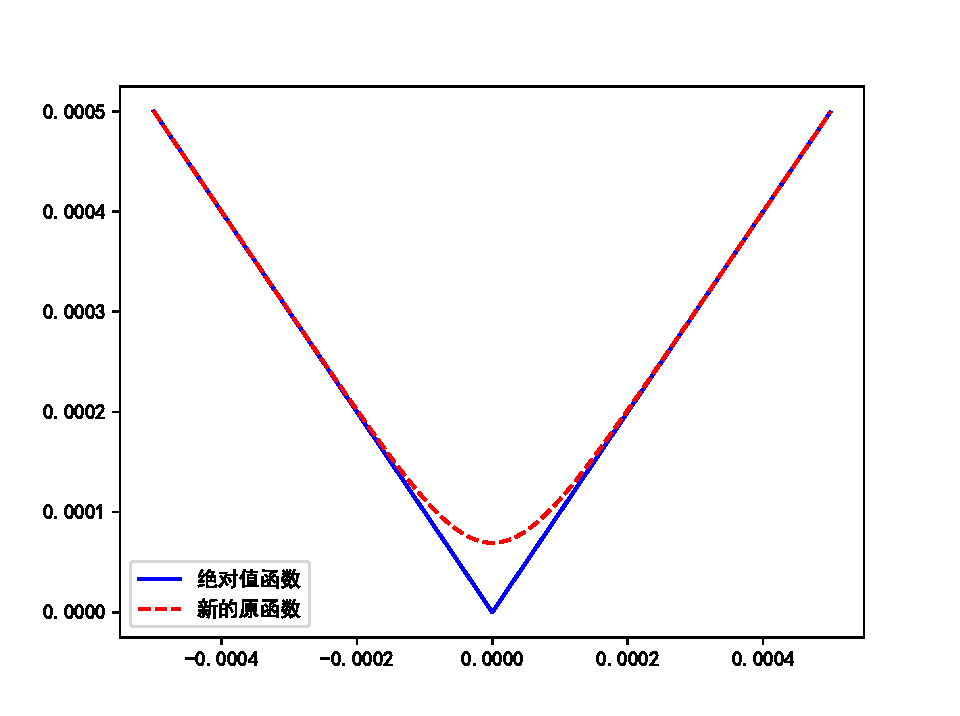
\includegraphics[width=\textwidth]{sgnVSnew.pdf}
	\caption{如图对比了${\left\| x \right\|}_1$和$\frac{1}{\beta}\mathbf{1}^T\mathrm{ln}\left[ \mathrm{cosh} \left( \beta x \right) \right] + \mathrm{ln}2$两种函数的差异,其中$\beta=10,000$。蓝色实线代表曼哈顿距离所基于的绝对值函数,红色虚线代表双曲正切函数的原函数。从图中可以看到,当$|x|>0.0002$时,二者已经几乎完全重合。}
	\label{fig:sgnVSnew}
\end{figure}

既然一阶导数和二阶导数已经由\eqref{eq:deri}和\eqref{eq:hessian}给出,$\mathcal{L}$可由牛顿法(Newton's Method)求解从而得到曼哈顿切线距离。我们把这个距离度量方式称为\textit{曼哈顿切线距离(Manhattan Tangent Distance, MTD)}。它的物理意义是对测试点和训练点所在的流形之间的曼哈顿距离的局部线性近似,也就是在切线上找到一点使得它到测试点的距离最小。

\subsection{低计算复杂度的近似解法}

虽然在上一节中我们提出了一种求解MTD的方法,但是该方法的缺点也是很明显的:过高的计算复杂度。该方法的时间复杂度是曼哈顿距离的$\mathcal{O}(NS)$倍,其中$N$是用有限差分法计算梯度所需的近邻数,$S$是牛顿法收敛所需的迭代步数。因为每次计算曼哈顿切线距离都需要迭代求解一个凸优化问题,若在线上系统中采用可能会有过高延迟。

因为切线距离是对物理空间中$\mathbf{x}$附近的点在信号空间中所形成的流形的局部线性近似,即\eqref{eq:mantd}中的切线距离只有在$a$接近0时才是对流形较好的估计。此外,我们注意到双曲正切函数$\mathrm{tanh}(x)$的一阶泰勒近似可写为$\mathrm{tanh}(x) = x + \mathcal{O}\left( x^3 \right)$。如果我们用$\mathrm{tanh}(x)$的一阶泰勒级数$x$代替它,则\eqref{eq:deri}中的$\frac{\partial \mathcal{L}}{\partial a}$将变为
\begin{equation}
\frac{\partial \mathcal{L}}{\partial a} = -\beta \mathbf{t}^T \left( \mathbf{s} - \mathbf{t}a - \widehat{\mathbf{s}} \right). \label{eq:approx}
\end{equation}
令\eqref{eq:approx}等于0的解和\eqref{eq:euca}一样。换句话说,近似算法中$a$的求解将采用和欧式切线距离相同的方法,但是将$a$带回目标函数计算切线距离时是基于曼哈顿距离的。我们把该算法叫做\textit{近似曼哈顿切线距离(Approximate Manhattan Tangent Distance, AMTD)}。

AMTD的时间复杂度是简单曼哈顿距离的$\mathcal{O}(N)$倍,相比于MTD,复杂度降低了$S$倍。

\section{实验与结果} \label{sec:exp}

\subsection{数据采集与预处理}

\begin{figure}[tb]
	\centering
	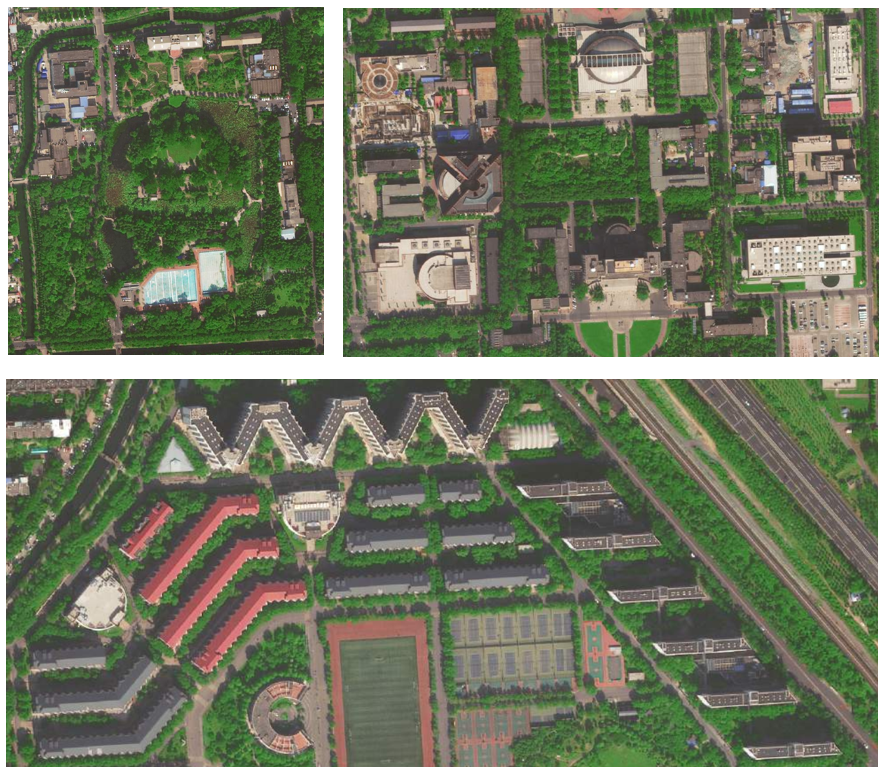
\includegraphics[width=\textwidth]{data_collection_area.png}
	\caption{如图所示为我们采集数据的三个区域的卫星图。左上子图为荷塘区域,右上子图为教学区,下子图为紫荆公寓区。}
	\label{fig:data_collection}
\end{figure}

这一节所用的数据由我们自己利用路测仪在清华大学校园内采集所得,路测仪在收集附近所有可接收信号基站的RSS的同时,还会收集GPS的定位信息。我们分别在三个不同的区域采集数据:
\begin{enumerate}
	\item 荷塘。这里是一个池塘,池塘中间有一个湖心岛,有很多树木但是没有高层建筑,如图\eqref{fig:data_collection}左上子图所示。这片区域总面积是$0.097\mathrm{km}^2$。数据由实验员手持路测仪步行采集,数据采集频率0.2Hz,两个时序相邻点的平均距离是5.0m。该数据集共有621个样本和85个可探测基站;
	\item 教学区。这片区域有一些高层建筑和树木,但是道路宽敞而且楼间距宽,如图\eqref{fig:data_collection}右上子图所示。这片区域总面积是$0.416\mathrm{km}^2$。数据由实验员骑车采集,路测仪采样频率0.5Hz。两个时序相邻点的平均距离是4.8m。该数据集共有2273个样本和204个可探测基站;
	\item 紫荆公寓区。这片区域有很多中层建筑而且道路狭窄,如图\eqref{fig:data_collection}下子图所示。这片区域总面积为$0.143\mathrm{km}^2$。数据由实验员骑车采集,路测仪采样频率0.5Hz。两个时序相邻点的平均距离是4.4m。该数据集共有1035个样本和149个可探测基站。
\end{enumerate}

虽然数据集中有很多可探测基站,但是对于每一条采样的接收信号来说,不会所有基站都有RSS,即数据会存在某些基站无接收信号的情况。为了应对这个问题,我们把每个基站的最小RSS减1作为缺省值。

\subsection{指数变换参数$\lambda$的选择} \label{subsec:lambda}

\begin{figure}[tb]
\centering
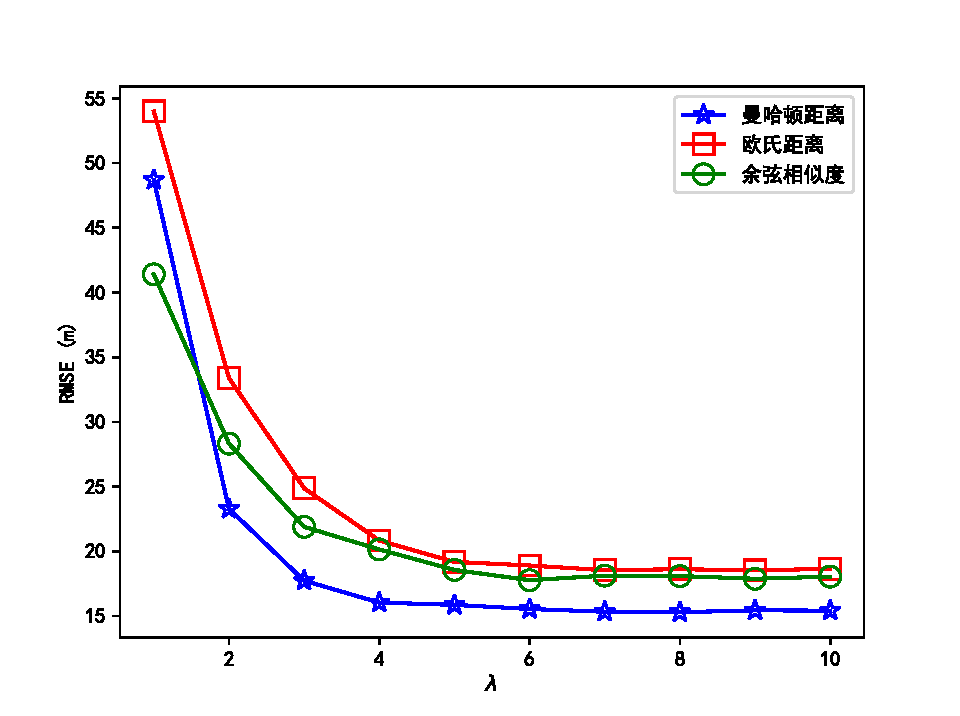
\includegraphics[width=\textwidth]{RMSE_lam.pdf}
\caption{如图所示为指数变换中参数$\lambda$与定位均方根误差RMSE的关系曲线,蓝色星形线是曼哈顿距离,红色方形线是余弦相似度,绿色圆形线是欧氏距离。当$\lambda>7$后RMSE几乎没有明显变化。}
\label{fig:rmse_lam}
\end{figure}

\begin{table}[tbp]
	\caption{指数变换后RMSE比较}
	\begin{center}
		\begin{tabular}{ccc}
			\toprule
			\textbf{RMSE/m} & \textbf{无指数变换} & \textbf{指数变换 ($\lambda=10$)} \\
			\midrule
			\textbf{曼哈顿距离} & 15.85 & 15.41 \\
			\midrule
			\textbf{欧氏距离} & 20.97 & 18.65 \\
			\midrule
			\textbf{余弦相似度} & 20.28 & 18.04 \\
			\bottomrule
		\end{tabular}
		\label{tab:no_exp}
	\end{center}
\end{table}

为了使定位效果最优,我们开展实验以找到指数变换中最优的$\lambda$参数,实验中KNN的参数k=3。对于不同的三种常用距离度量方式,画出$\lambda$与RMSE之间的关系曲线,如图\ref{fig:rmse_lam}所示。这里只有从荷塘采集的数据参与了实验,一是为了减少计算时间,二是防止过拟合,即后两个数据集没有参与参数$\lambda$的调节,而是直接使用。为了尽可能消除噪声的影响并使曲线平滑,对于每个$\lambda$均随机选取10\%的数据作为测试数据并随机进行1000次。从图中可以看出当$\lambda>7$后RMSE几乎没有明显变化,因此在后续实验中我们将令$\lambda=10$。

作为对比,不采用指数变换的指纹定位效果在表\ref{tab:no_exp}中给出,其中指数变换的$\lambda=10$。实验结果显示指数变换的确可以一定程度上提高定位精度。

此外,很明显曼哈顿距离可以取得最小的定位误差,因此在我们的数据集下,最常用的欧氏距离并不是最优选择。至于余弦相似度,它的表现比欧氏距离好,但是依然劣于曼哈顿距离。

\subsection{KNN中近邻数k的选择}

\begin{figure}[tb]
	\centering
	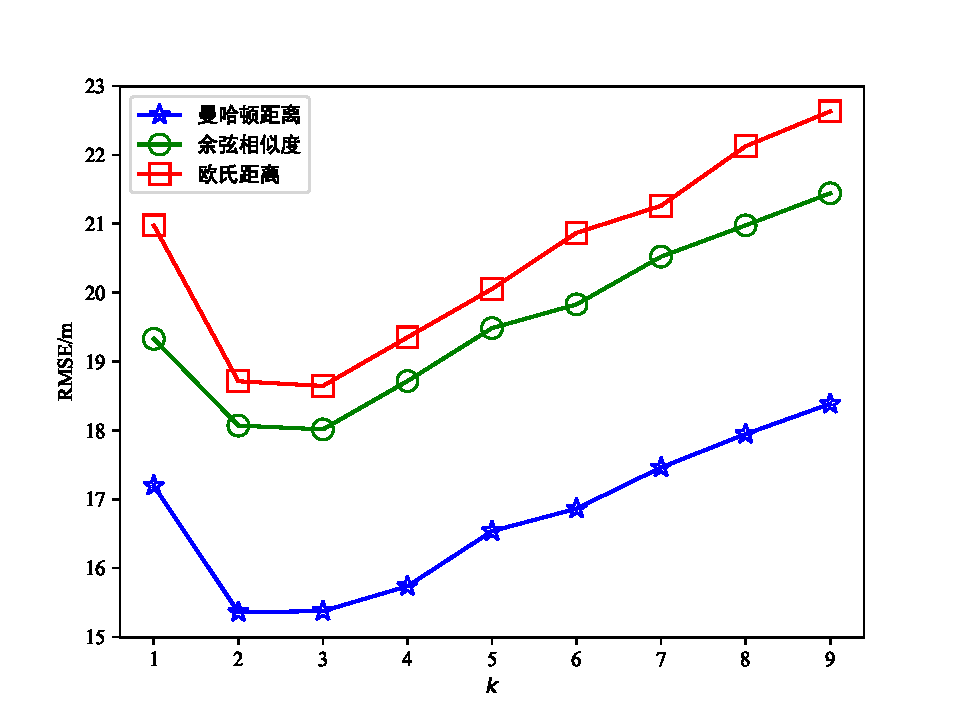
\includegraphics[width=\textwidth]{RMSE_k.pdf}
	\caption{如图所示为KNN中参数$k$与定位均方根误差RMSE的关系曲线,蓝色星形线是曼哈顿距离,绿色圆形线是余弦相似度,红色方形线是欧氏距离。当$k$取2或3时可以取得最小定位误差。}
	\label{fig:rmse_k}
\end{figure}

此处仍然只使用荷塘的数据。在$\lambda=10$的条件下,针对不同的参数$k$开展实验,测试集的选取和实验次数与第\ref{subsec:lambda}节的设置相同。实验结果如图\ref{fig:rmse_k}所示。对于三种度量方式来说,都是在$k$=2或3时RMSE最小,因此在后续的实验中我们将把$k$固定为3。

\subsection{切线距离的导数中参数$N$的选择}

\begin{figure}[tb]
	\centering
	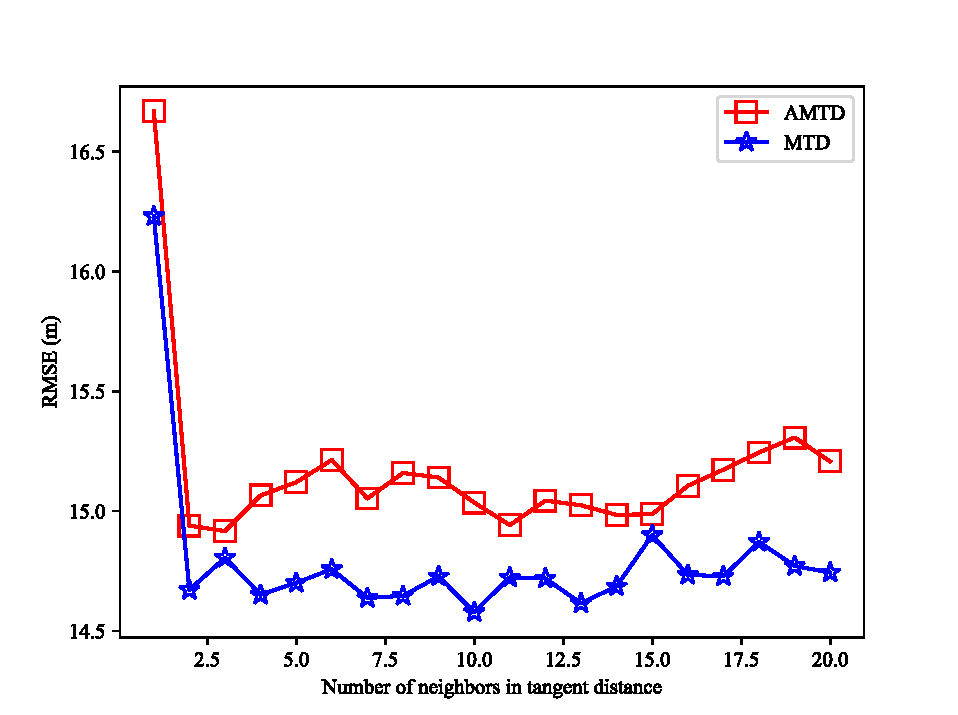
\includegraphics[width=\textwidth]{RMSE_N.pdf}
	\caption{如图所示为求解切线距离时求导数所需近邻数$N$与定位均方根误差RMSE的关系曲线,蓝色星形线是曼哈顿切线距离MTD,红色方形线是近似曼哈顿切线距离AMTD。由于实验次数少导致曲线波动较大,不过大致可以看出当$N>2$时几乎没有太大的变化。}
	\label{fig:rmse_n}
\end{figure}

这里依然只使用荷塘的数据。这里使用K-fold方法,即将数据集随机分成k份,之后循环k次,依次取一份作为测试数据,其余k-1份作为训练数据。在该实验中k=10即每次取10\%的数据作为测试数据。每个fold中,MTD和AMTD将同时训练和测试。在MTD中,牛顿法的停止判据是$10^{-4}$。

图\ref{fig:rmse_n}是实验结果。虽然由于实验次数少导致曲线一直在抖动,但是总体趋势大致是先急剧下降,在$2 \le N \le 15$的范围内基本不变,之后缓慢上升。在综合考虑精度和计算复杂度后,我们决定在后续实验中将$N$设为5。

\subsection{切线距离定位效果}

\begin{table}[tbp]
	\caption{切线距离定位效果对比}
	\begin{center}
		\begin{tabular}{cccc}
			\toprule
			RMSE/m &  荷塘 & 教学区 & 公寓区 \\
			\midrule
			欧氏距离 & 19.20 & 13.56 & 10.29 \\
			\midrule
			ETD & 16.69 & 11.47 & 9.54 \\
			\midrule
			曼哈顿距离 & 15.78 & 9.96 & 7.95 \\
			\midrule
			\textbf{MTD} & \textbf{14.75} & \textbf{9.14} & \textbf{7.45} \\
			\midrule
			\textbf{AMTD} & \textbf{14.90} & \textbf{9.43} & \textbf{7.63} \\
			\bottomrule
		\end{tabular}
		\label{tab:td}
	\end{center}
\end{table}

\begin{table}[tbp]
	\caption{切线距离定位效果对比}
	\begin{center}
		\begin{tabular}{cccc}
			\toprule
			RMSE相对减少 &  荷塘 & 教学区 & 公寓区 \\
			\midrule
			ETD & -13.1\% & -15.4\% & -7.29\% \\
			\midrule
			MTD & -6.53\% & -8.23\% & -6.29\% \\
			\midrule
			AMTD & -5.58\% & -5.32\% & -4.03\% \\
			\bottomrule
		\end{tabular}
		\label{tab:td_relative}
	\end{center}
\end{table}

综合上述实验的结论,我们令指数变换参数$\lambda=10$,KNN中的参数$k=3$。涉及切线距离时,计算导数所需的近邻数$N$设为5。这些参数将被用于加权-KNN中,分别以欧式距离、欧式切线距离、曼哈顿距离、曼哈顿切线距离和近似曼哈顿切线距离作为距离度量方式,比较和分析定位效果。

实验结果展示在表\ref{tab:td}中。首先,注意到欧式切线距离ETD可以取得比欧氏距离更小的RMSE,但是仍然高于简单的曼哈顿距离,这也是我们提出曼哈顿切线距离MTD的动机。其次,实验结果显示MTD在所有三个数据集中均取得最小的RMSE。除此之外,虽然近似曼哈顿切线距离AMTD的RMSE略高于MTD,但是仍然低于曼哈顿距离的RMSE而且在我们的实验中效果仅次于MTD,而且计算复杂度远小于MTD。相比于曼哈顿距离,在三个数据集中,ETD相比于欧氏距离、MTD和AMTD相比于曼哈顿距离的相对RMSE减少如表\ref{tab:td_relative}所示。显然,无论对于ETD、MTD还是AMTD来说,都是从公寓区采集的数据定位精度的相对提升幅度最小。我们分析可能的原因是公寓区采集的数据其时序相邻点的平均距离最小,因此相比于其他数据集,像欧氏距离和曼哈顿距离等简单距离度量方式能够更好的估计流形之间的距离。但是定位精度会受到很多其他因素影响,比如阴影效应和多径效应等。相比于其他区域,公寓区的建筑较高而且密集,存在较多的遮挡以及散射路径,这可能导致距离的小幅变化反映到信号空间会变化较大,这也会限制切线距离的提升效果。

\section{本章小结}

这一章我们讨论了将切线距离应用于基于接收信号强度和加权-KNN的指纹定位算法中。首先,我们简单介绍了指纹定位的KNN算法中常见的距离度量方式,并分析了他们的缺点,包括给予不同大小的接收信号强度相同的权重以及在流形存在的情况下简单度量方式不能反映真实距离等问题。针对这些问题,我们分别利用指数变换和切线距离来解决。其后,我们阐明了切线距离背后所蕴含的思想,并介绍了原作者所提出的基于欧氏距离的切线距离ETD。然而,因为在实测数据实验中欧式切线距离的定位效果虽然相较于欧氏距离有提升,但是依然劣于曼哈顿距离,于是我们提出了曼哈顿切线距离MTD以及在定位精度和计算复杂度之间折中的近似曼哈顿切线距离AMTD。为了验证算法性能,我们在清华大学校园内不同的三个区域采集数据,开展实验找到适合的KNN近邻数$k$、指数变换参数$\lambda$以及切线距离中计算导数所需的近邻数$N$。最后,我们比较了欧氏距离、ETD、曼哈顿距离、MTD和AMTD的定位误差RMSE。在所有三个数据集中,MTD均取得了最小的定位误差,而AMTD则以远小于MTD的计算量取得了仅次于MTD却依然优于曼哈顿距离的定位精度。





